\documentclass[a4paper,titlepage]{article}

\makeatletter
\def\input@path{{../../../template/}{./img}}
\makeatother

\usepackage{Comandi}
\usepackage{Riferimenti}
\usepackage{Stile}

\usepackage{eurosym}
\usepackage{comment}
\usepackage{hyperref}

\def\NOME{Specifica Tecnica}
\def\VERSIONE{1.0.0}
\def\DATA{2016-06-xx}
\def\REDATTORE{Viviana Alessio \\ & Matteo Franco \\ & Andrea Grandene \\ & Luca Soldera}
\def\VERIFICATORE{Enrico Bellio \\ & Tommaso Panozzo}
\def\RESPONSABILE{Matteo Franco}
\def\USO{Esterno}
\def\DESTINATARI{\COMMITTENTE \\ & \CARDIN \\ & \PROPONENTE}
\def\SOMMARIO{Descrizione dell'architettura ad alto livello per il \gl{progetto} \PROGETTO.}


\begin{document}


\maketitle

\begin{diario}
	\modifica{Matteo Franco}{\PRJ}{Stesura intestazione documento}{2016-05-23}{0.0.1}
\end{diario}

\newpage
\tableofcontents
\newpage
\listoftables
\newpage
\listoffigures
\newpage

\section{Introduzione}
	\subsection{Scopo del documento} 
	Questo documento ha lo scopo di spiegare dettagliatamente le strategie secondo cui il gruppo \AUTORE{} intende condurre il \gl{progetto} didattico. 
	\subsection{Scopo del \gl{prodotto}}
	\SCOPO
	\subsection{Glossario}
	\GLOSSARIO
	\subsection{Riferimenti}
		\subsubsection{Normativi}
			\begin{itemize}
				\item \textbf{Capitolato d'appalto C2 - CLIPS:} Communication \& Localisation with Indoor Positioning Systems. \\
				\url{http://www.math.unipd.it/~tullio/IS-1/2015/Progetto/C2.pdf}
				\item \textbf{Vincoli e dettagli tecnico-economici} \\
				\url{http://www.math.unipd.it/~tullio/IS-1/2015/Dispense/PD01.pdf}
				\item \textbf{Norme di Progetto} \\ \NPdoc
				\item \textbf{Regolamento di Progetto} \\
				\url{http://www.math.unipd.it/~tullio/IS-1/2015/Progetto/}
				\item \textbf{Regolamento organigramma} \\
				\url{http://www.math.unipd.it/~tullio/IS-1/2015/Progetto/PD01b.html}
			\end{itemize}	
			
		\subsubsection{Informativi}
			\begin{itemize}
				\item \textbf{Software Engineering (10th edition}) \\
				Ian Sommerville \\
				Pearson Education | Addison-Wesley
				\item \textbf{Guide to the Software Engineering Body of Knowledge}
				IEEE Computer Society. Software Engineering Coordinating Committee
				\item \textbf{Slides del \COMMITTENTE} \\ riguardo i  \href{http://www.math.unipd.it/~tullio/IS-1/2015/Dispense/L02.pdf}{processi \gl{software}}, il \href{http://www.math.unipd.it/~tullio/IS-1/2015/Dispense/L03.pdf}{ciclo di vita del \gl{software}} e \href{http://www.math.unipd.it/~tullio/IS-1/2015/Dispense/L04.pdf}{la gestione di \gl{progetto}}	
			\end{itemize}
	\subsection{Modello di ciclo di vita scelto}
	È stato scelto come ciclo di vita il modello \gl{incrementale}. Le motivazioni che ci hanno spinto verso questa direzione sono il modo in cui è strutturato il \gl{progetto} didattico e la quasi totale inesperienza dei componenti del gruppo nello sviluppare progetti \gl{software} di grandi dimensioni. Di seguito una lista di caratteristiche del metodo \gl{incrementale}:
	\begin{itemize}
		\item si può produrre valore ad ogni incremento;
		\item ogni incremento riduce il rischio di fallimento;
		\item prevede rilasci multipli;
		\item i requisiti utente sono classificati e trattati in base alla loro importanza strategica. I requisiti più importanti sono già stabili all'inizio dello sviluppo del \gl{progetto};
		\item l'analisi dei requisiti e la progettazione architetturale non vengono ripetute;
		\item prima si pensa allo sviluppo dei requisiti essenziali, poi a quelli desiderabili;
		\item Sono presenti delle iterazioni del tipo Prototipo $\rightarrow$ Validazione $\rightarrow$ Prototipo $\rightarrow$ Validazione $\rightarrow$ ecc..
	\end{itemize}
	\subsection{Scadenze}
	Il gruppo Beacon Strips ha deciso di rispettare le seguenti scadenze:
	\begin{itemize} 
		\item \textbf{Revisione dei Requisiti}: 2016-04-18
		\item \textbf{Revisione di Progettazione}: 2016-06-17
		\item \textbf{Revisione di Qualifica}: 2016-08-24
		\item \textbf{Revisione di Accettazione}: 2016-09-12
	\end{itemize}
	In base a queste scadenze e a fronte dell'analisi dei rischi verranno decise le fasi in cui suddividere il lavoro di sviluppo del \gl{progetto}.
	\subsubsection{Scelta Revisione di Progettazione}
	Si è deciso di affrontare la RP$_{\mbox{\textit{min}}}$. Il gruppo si impegna quindi per il 2016-06-17 di presentare nel documento ``Specifica Tecnica'' la progettazione ad alto livello del \gl{prodotto}.
	

\section{Tecnologie utilizzate} 
Per lo sviluppo del progetto abbiamo la necessità di utlizzare delle tecnologie che sono state scelte dopo attenta analisi. 


\section{Descrizione architettura} 
\label{architettura}
	In questa sezione verrà descritta lo schema generale dell'architettura, nella sezione successiva % aggiungere label
	verranno riportate tutti i packages e le classi dettagliatamente.
	 Per i diagrammi delle classi e di attività è stato utilizzato il formalismo UML 2.0. \\
	 L'architettura descritta in questo documento è ad alto livello. Classi, sottoclassi e attributi verranno descritti più dettagliatamente nel periodo in cui attueremo la Progettazione di dettaglio. \\
	 Si procederà nella descrizione dell'architettura con un approccio top-down. Saranno descritte prima quindi le parti più generali per poi andare sempre più nello specifico. Si procederà quindi prima con la descizione dei packages e delle componenti, per poi passare alle singole classi. Successivamente verranno descritti i design pattern utilizzati.
	
	\subsection{Architettura generale}
	L'architettura generale dell'applicazione segue il modello client - server. \\
	In particolare si utilizzerà lo stile architetturale REST (representational state transfer) per coordinare compomenti, connettori e dati attraverso un sistema ipermediale distribuito dove l'attenzione è data al ruolo delle componenti.
	
	\begin{itemize}
		\item \textbf{Vantaggi}: REST offre una interfaccia che separa il client dal server. Questa separazione 
	\end{itemize}
		
		rest - A uniform interface separates clients from servers. This separation of concerns means that, for example, clients are not concerned with data storage, which remains internal to each server, so that the portability of client code is improved. Servers are not concerned with the user interface or user state, so that servers can be simpler and more scalable. Servers and clients may also be replaced and developed independently, as long as the interface between them is not altered.

% package
% \include{package}

% classi
% \include{classi}

\section{Diagrammi delle attività} 
\label{attivita}
I diagrammi delle attività realizzati mostrano in dettaglio i flussi di azioni che un utente può svolgere all'interno dell'applicazione. \\
Alcuni diagrammi contengono azioni che sono a loro volta state descritte dettagliatamente in altri diagrammi di attività. Per migliorare la comprensibilità queste azioni sono state differenziate dalle altre inserendovi uno sfondo colorato.
\subsection{Avvio}
Questo diagramma contiene tutte le azioni che l'utente può svolgere all'interno dell'applicazione. \\

\subsection{Registrazione}
L' utente può registrarsi al sistema inserendo tutti i campi nel form che gli si presenterà davanti una volta cliccato il pulsante ``Registrati'' dal menu dell'applicazione. È previsto l'inserimento obbligatorio di tutti i campi del form.
I campi che l'utente deve riempire sono i seguenti:
\begin{itemize}
	\item Indirizzo email;
	\item Username;
	\item Password;
	\item Reinserimento password;
\end{itemize}
Subito dopo che l'utente riempirà un campo della form verrà subito notificato in caso i dati inseriti non fossero validi. \\
Una volta che tutti i dati saranno inseriti correttamente l'utente potrà confermare i dati e verrà automaticamente autenticato nel sistema.

\subsection{Login}
L'utente che si è già registrato e vuole autenticarsi nel sistema deve effettuare il login. \\
Nel caso l'utente ricordi i propri dati per accedere seguirà il ramo sinistro del primo punto di decisione del diagramma. Una volta entrato nella pagina di login inserirà nell'apposito form il proprio indirizzo email e la propria password. Successivamente confermerà i propri dati. Se entrambi i campi sono stati riempiti correttamente l'utente sarà autenticato altrimenti gli viene data l'opportunità di reinserire i dati oppure di effettuare il recupero password. \\
Nel caso l'utente non ricordi le proprie credenziali di accesso può richiedere una nuova password, seguirà quindi il ramo destro del primo punto di decisione del diagramma. Per ottenere una nuova password basterà che inserisca la propria email. Se tale indirizzo è presente nel database del sistema verrà inviata ad esso una email contenente una nuova password. Una volta ricevuta l'email l'utente può tornare nell'applicazione ed effettuare il login seguendo il ramo sinistro del primo punto di decisione del diagramma.

\subsection{Modifica credenzali}
Un utente autenticato può modificare alcune delle sue credenziali. In particolare potrà modificare il proprio username e/o la propria password.
Viene eseguito un controllo di correttezza dei dati inseriti dopo ogni inserimento come avviene per durante la registrazione.

\subsection{Percorsi}
Un utente autenticato può decidere di intraprendere un percorso. \\ 
Innanzitutto sceglierà il percorso che desidera fare e successivamente potrà iniziare a svolgerlo. \\ Un percorso si compone di una serie di tappe che prevedono il susseguirsi dei seguenti passi:
\begin{itemize}
	\item Ricerca beacon;
	\item Trovato beacon;
	\item Visualizza istruzioni prova;
	\item Svolgimento prova;
	\item Visualizza risultato prova.
\end{itemize}
L'utente continuerà a svolgere queste azioni finchè il percorso non sarà concluso. Successivamente visualizzerà il riepilogo dei dati del percorso appena concluso e potrà decidere se salvare oppure no i dati che ha appena visualizzato. Quest'ultima operazione sarà possibile solo se l'utente è autenticato, quindi gli viene data a possibilità a questo punto sia di effettuare il login sia di effettuare la registrazione.

\subsection{Ricerca edifici}
L'utente può cercare edifici vicini alla posizione in cui si trova. \\ 
Se si trova in un edificio abilitato visualizzerà direttamente le informazione dell'edificio stesso e successivamente si potrà cercare altri edifici nelle vicinanze. \\ 
Se non si trova in nessun edificio abilitato potrà visualizzare la lista degli edifici più vicini. Se lo desidera si potrà inserire un raggio di ricerca e visualizzare quindi solo gli edifici che gli interessano. \\
Ogni elemento presente nella lista è cliccabile e, una volta cliccato, manderà l'utente in una pagina dove visualizzerà tutti i dettagli dell'edificio e i suoi relativi percorsi.


\section{Stime di fattibilità} 


% tracciamento 
% \include{tracciamento}

\appendix
\newcommand{\utilizzo}{\item \textbf{Utilizzo nel progetto}}

\section{Design pattern utilizzati}
\label{pattern}
\subsection{Pattern architetturali}
	\subsubsection{Model View Controller}
	
		\begin{figure}[!h]
			\centering
			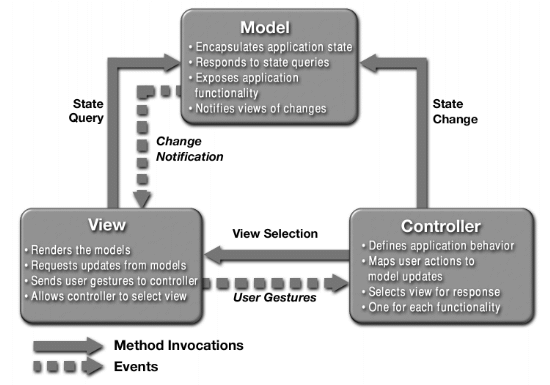
\includegraphics[scale=0.5]{img/mvc}  
			\caption{Struttura del pattern MVC}
		\end{figure}
		
		\begin{itemize}	
			\item \textbf{Descrizione} \\ Model View Controller è un design pattern architetturale che permette di dividere l'architettura del sistema che si intende sviluppare in tre blocchi:
			\begin{itemize}
				\item \textbf{il modello} che contiene le classi con i metodi di accesso ai dati;
				\item \textbf{la vista} che contiene le classi che permettono all'utente di visualizzare i dati e di interagire con il modello;
				\item \textbf{il controllore} che si occupa di fare da tramite tra vista e modello, ovvero riceve i comandi dell'utente attraverso la vista e va a cambiare lo stato del modello di conseguenza, successivamente aggiorna la vista.				
			\end{itemize}
			
			\item \textbf{Vantaggi} \\
			Questo pattern architetturale permette il riuso del codice in quanto molte parti di lavoro sono indipendenti. Ad esempio il modello creato potrà essere utilizzato con diverse viste. \\ Grazie all'indipendenza di alcune parti è semplice dividere il lavoro tra più componenti di un team e sarà quindi più facile anche la manutenzione.
			\utilizzo \\
			Nel nostro progetto il pattern MVC è usato nella parte client dell'architettura. 
		\end{itemize}
		
		\newpage
		
\subsection{Pattern creazionali}
	\subsubsection{Abstract Factory}
	
	\begin{figure}[!h]
		\centering
		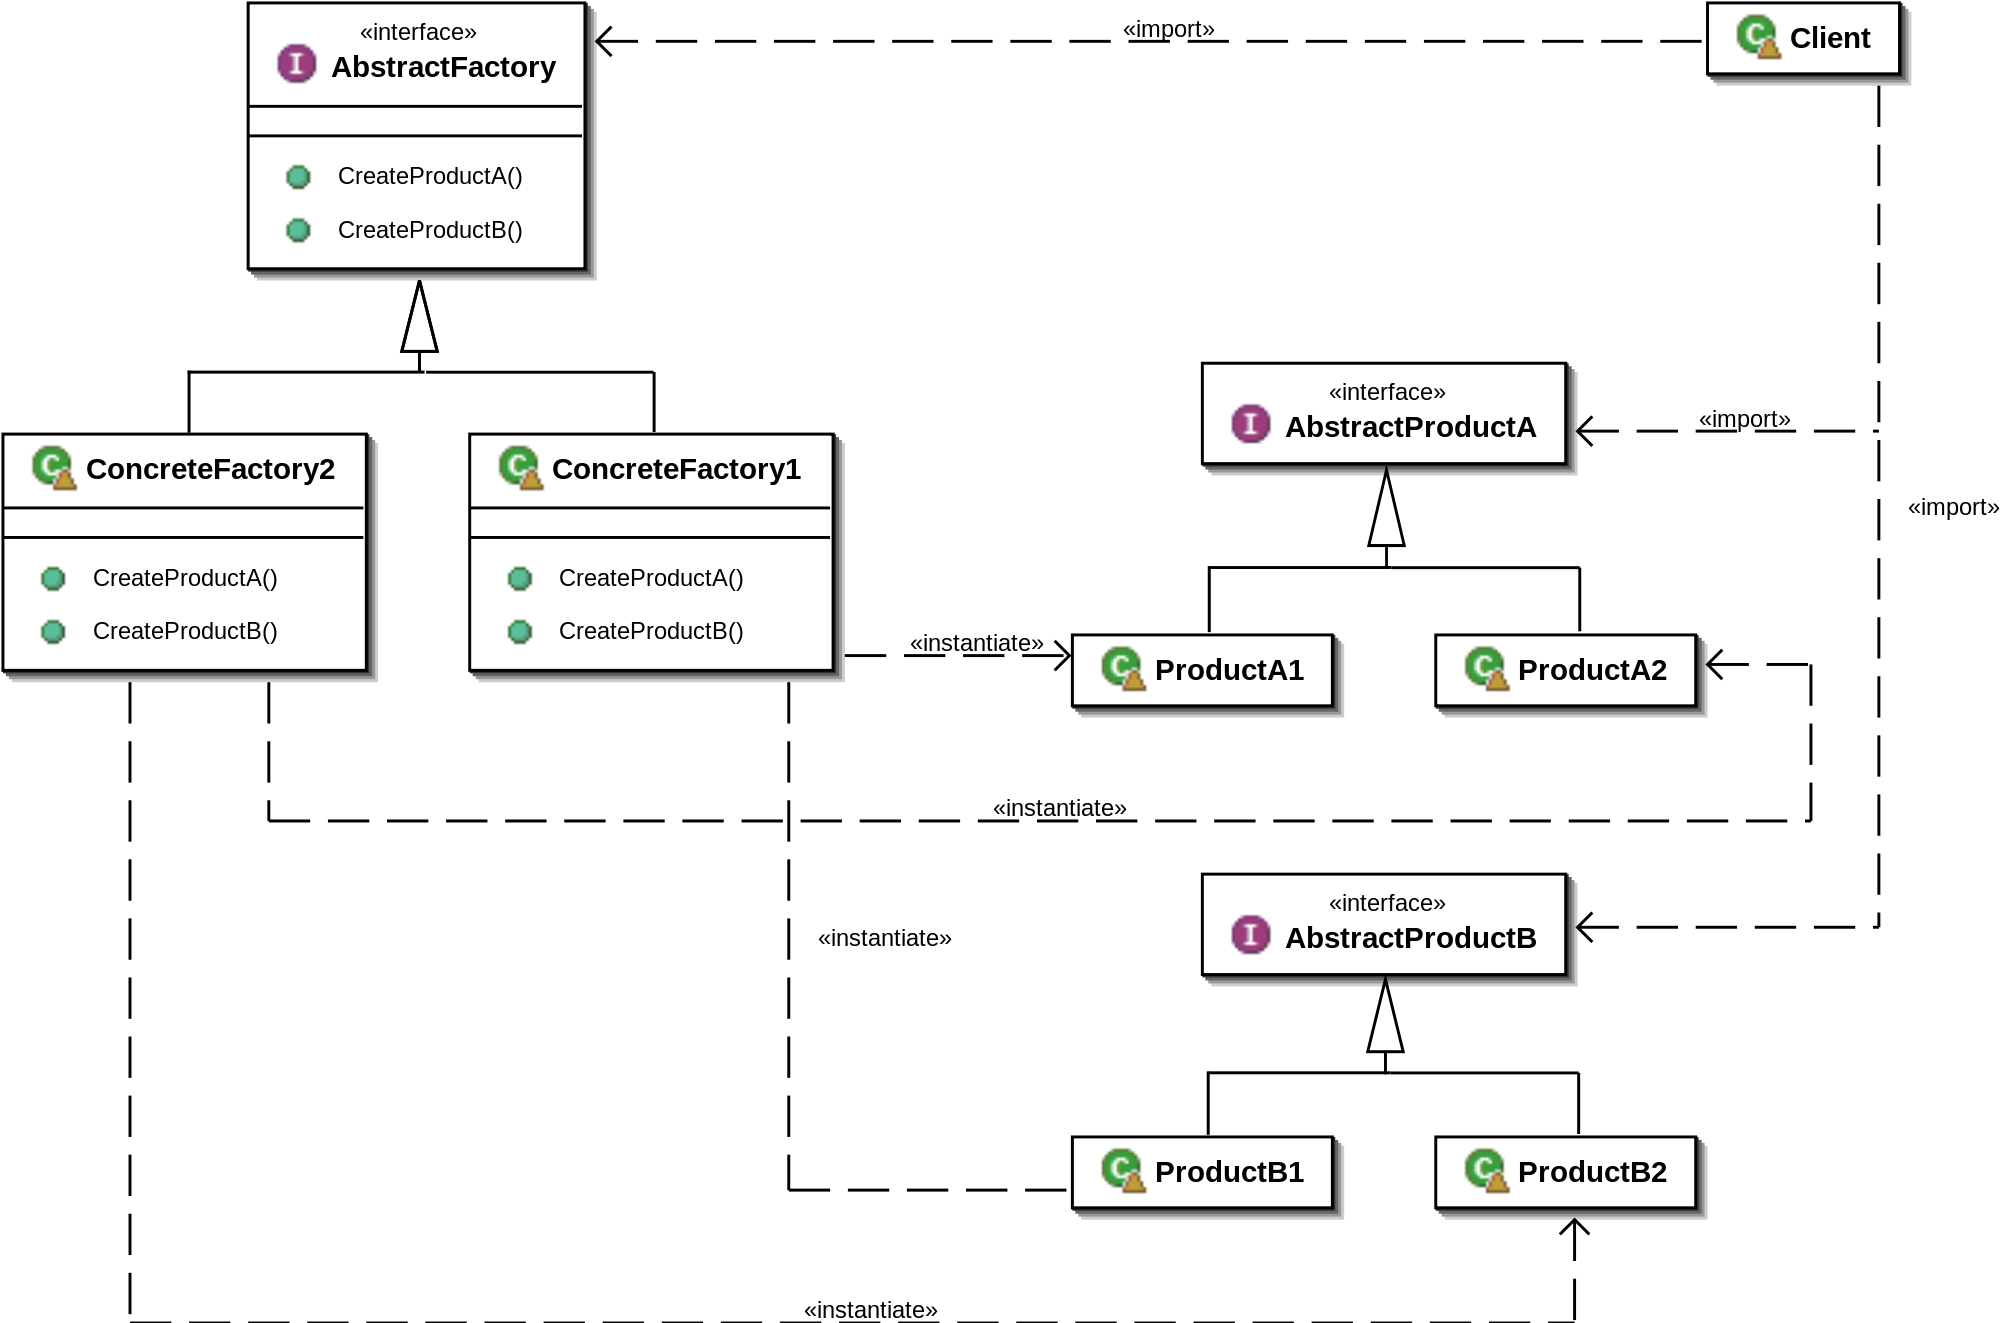
\includegraphics[scale=0.2]{img/abstract_factory}  
		\caption{Struttura del pattern Abstract Factory}
	\end{figure}
	
		\begin{itemize}
			\item \textbf{Descrizione}\\ 
			Il design pattern Abstract Factory fornisce un'interfaccia per creare famiglie di prodotti senza specificare classi concrete. Ogni famiglia di prodotti ha una classe base astratta da cui derivano delle classi concrete. Queste classi concrete sono istanziate dalle classi concrete della factory corrispondenti.
			% immagine di esempio
			
			\item \textbf{Vantaggi}\\ 
			Questo design pattern offre vantaggi quando si vogliono modellare famiglie di prodotti che potranno essere ampliate nel futuro. Le modifiche necessarie ad aggiungere nuovi elementi alle famiglie saranno essenzialmente due, aggiungere una classe in ogni famiglia di prodotti ed un solo metodo nella factory.
			\utilizzo \\ 
			Nel nostro progetto abbiamo utilizzato questo design pattern per modellare i tipi di quiz che vengono proposti agli utenti. Abbiamo infatti deciso di utilizzare solo due famiglie di quiz, quindi vi è la necessità di avere modo in futuro di ampliare le tipologie di quiz disponibili in modo semplice ed efficace.
			
			\begin{figure}[!h]
				\centering
				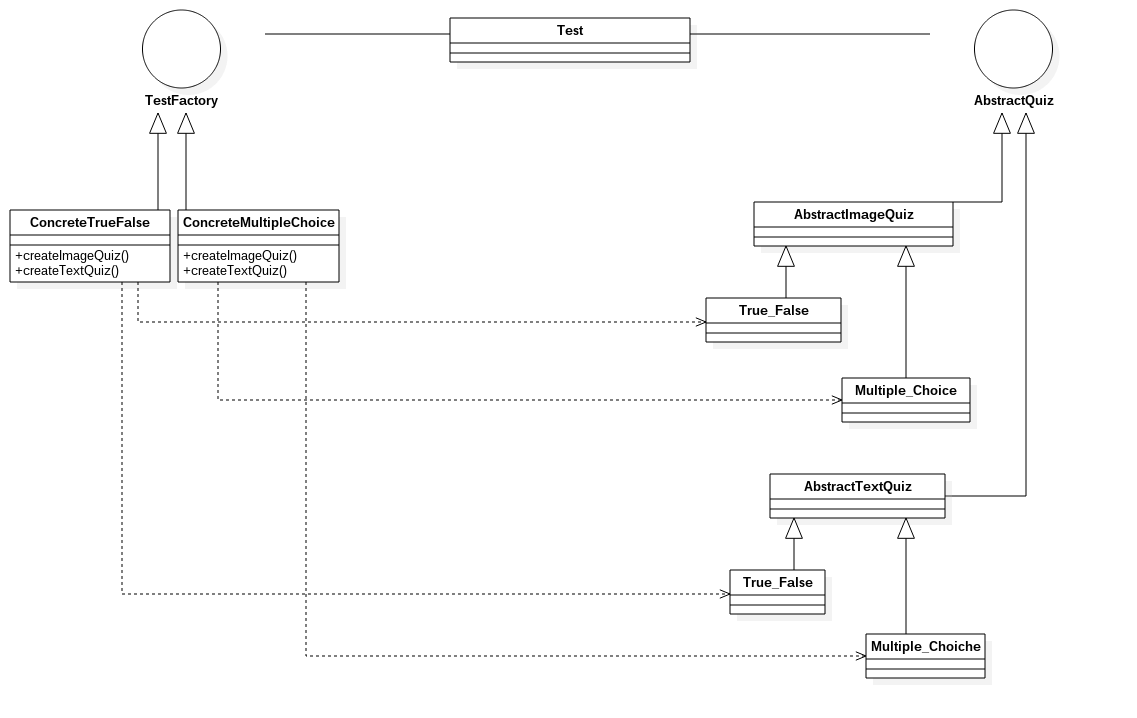
\includegraphics[scale=0.4]{img/our_abstract_factory}  
				\caption{Utilizzo di Abstract Factory nel progetto}
			\end{figure}
			
		\end{itemize}
	 \newpage
	 
	\subsubsection{Singleton}
		\begin{figure}[!h]
			\centering
			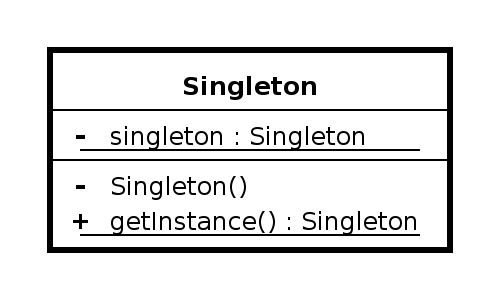
\includegraphics[scale=0.4]{img/singleton}  
			\caption{Struttura del pattern Singleton}
		\end{figure}
		
		\begin{itemize}
			\item \textbf{Descrizione}\\ 
			 Assicura l'esistenza di un'unica istanza di una classe e permette di avere un punto di accesso globale a questa.
			 Per rendere possibile ciò si mette il costruttore protetto o privato e si crea un metodo statico, chiamato factory, che fornisce l’accesso all'unica copia dell’oggetto (contiene un puntatore all’unica istanza).			 
			 \item \textbf{Vantaggi}\\ 
			 Se, al contrario di quanto avviene utilizzando Singleton, venisse reso visibile il costruttore della classe non si potrebbe garantire che esista un solo esemplare della classe. Un altro modo di procedere potrebbe essere quello di dichiarare una variabile globale, ma in questo modo si ``ruberebbe'' un nome al namespace globale.
			 Sigleton permette inoltre di dichiarare sottoclassi.			 
			 \utilizzo \\ 
			 Nel nostro progetto abbiamo creato un singleton per ``LoginManager'' che contiene i dati relativi a i dati di login dell'utente che sta utilizzando l'applicazione.
			 
			 	\begin{figure}[!h]
			 		\centering
			 		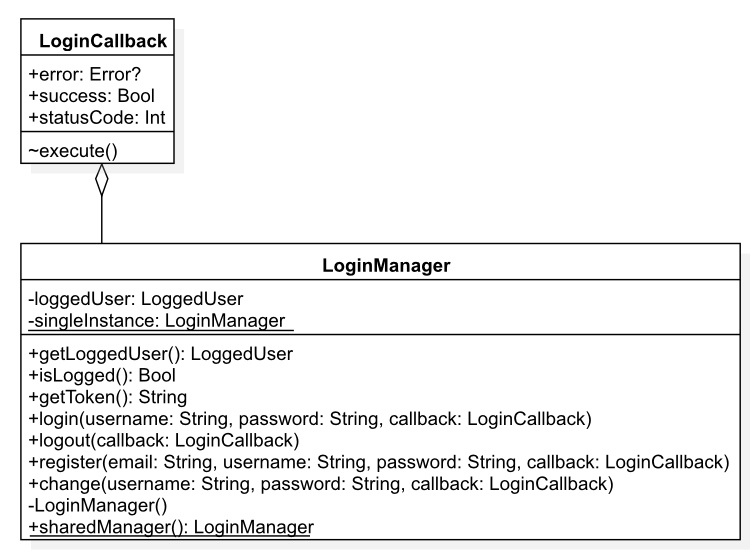
\includegraphics[scale=0.4]{img/package/png/client--loginmanager}  
			 		\caption{Utilizzo di Abstract Factory nel progetto}
			 	\end{figure}
			 
		\end{itemize}
		
		
		


\end{document}
